\documentclass[xcolor={table}]{beamer}


\usepackage[T1]{fontenc}
\usepackage[utf8]{inputenc}
\usepackage{lmodern}
%%%%%%%%%%%%%%%%%%%%%%%%%%%%%%%%%%%%%%%%%%%%%%%%%%%%%%%%%
% Source: http://en.wikibooks.org/wiki/LaTeX/Hyperlinks %
%%%%%%%%%%%%%%%%%%%%%%%%%%%%%%%%%%%%%%%%%%%%%%%%%%%%%%%%%
\usepackage{hyperref}
\usepackage{graphicx}
\usepackage[english]{babel}

\usepackage{bm}
\usepackage{amsmath}
\usepackage{amsfonts}

\usepackage{amsthm}
\newtheorem{definition}{Definizione}
\newtheorem{theorem}{Teorema}
\renewcommand*{\proofname}{Dimostrazione}
\newtheorem{example}{Esempio}
\newtheorem{lemma}{Lemma}
\newtheorem{exercise}{Esercizio}
\newtheorem{property}{Proprietà}

\usepackage[ruled,vlined,linesnumbered]{algorithm2e}

\newcommand{\xstar}{x^*}
\newcommand{\bxstar}{\bm{x^*}}
\newcommand{\bx}{\bm{x}}
\newcommand{\Rn}{\mathbb{R}^n}
\newcommand{\RR}{\mathbb{R}}
\newcommand{\norm}[1]{\left\lvert \left\lvert #1 \right\lvert \right\lvert}

\newcommand{\fx}{f(x)}

\newcommand{\gradfx}{\nabla \fx}
\newcommand{\Gx}{\nabla f(x)}
\newcommand{\Gk}{\nabla f(x_k)}
\newcommand{\Gs}{\nabla f(\xstar)}

\newcommand{\Hx}{\nabla^2 f(x)}
\newcommand{\Hk}{\nabla^2 f(x_k)}
\newcommand{\Hs}{\nabla^2 f(\xstar)}
\newcommand{\hess}{\nabla^2 f}

\newcommand{\step}{\alpha}
\newcommand{\Seqx}{\{ x_k \}}

\usepackage{mathtools}
\newcommand\myeq{\stackrel{\mathclap{\normalfont\mbox{def}}}{=}}

\usepackage{listings}
\lstset
{ 
    language=Matlab,
    basicstyle=\normalsize,
    numbers=left,
    stepnumber=1,
    showstringspaces=false,
    tabsize=1,
    breaklines=true,
    breakatwhitespace=false,
   frame=single
}


\usepackage{amsmath}
\usepackage{beamerthemesplit}
\usepackage{graphicx}
\usepackage{epsfig}
\usepackage{color}
\usepackage{multirow}
\usepackage[ruled,vlined]{algorithm2e}
\usepackage{lmodern}
\usepackage[round]{natbib}
\usepackage{fancybox}

%%% MY COMMANDS
\newcommand{\nota}[1]{{\bf [#1]}}
\newcommand{\reff}[1]{(\ref{#1})}
\newcommand{\obar}[1]{\overline{#1}}
\newcommand{\ubar}[1]{\underline{#1}}
\newcommand{\ceil}[1]{\lceil #1 \rceil}
\newcommand{\floor}[1]{\lfloor #1 \rfloor}
\newcommand{\ie}{{\it i.e.}}
\newcommand{\vx}{{\bf x}}
\newcommand{\vy}{{\bf y}}
\newcommand{\vb}{{\bf b}}
\newcommand{\vc}{{\bf c}}
\newcommand{\va}{{\bf a}}
\newcommand{\vpi}{{\bf \pi}}

\newcommand{\myf}[1]{\textcolor{red}{{\mathnormal f}\big( #1 \big)}}
\newcommand{\myF}[1]{\textcolor{red}{{\mathnormal f}\bigg( #1 \bigg)}}

\definecolor{darkgreen}{rgb}{0,0.4,0}

\newcommand{\tb}[1]{\textcolor{blue}{#1}}
\newcommand{\tre}[1]{\textcolor{red}{#1}}
\newcommand{\tgrey}[1]{\textcolor{grey}{#1}}
\newcommand{\tgr}[1]{\textcolor{darkgreen}{#1}}
\newcommand{\tye}[1]{\textcolor{yellow}{#1}}
\newcommand{\cya}[1]{\textcolor{cyan}{#1}}
\newcommand{\cnt}[1]{{\tt \textcolor{cyan}{#1}}}
\newtheorem{proposition}{Proposition}[section]

\newenvironment{changemargin}[2]{% 
    \begin{list}{}{% 
            \setlength{\topsep}{0pt}% 
            \setlength{\leftmargin}{#1}% 
            \setlength{\rightmargin}{#2}% 
            \setlength{\listparindent}{\parindent}% 
        \setlength{\itemindent}{\parindent}% 
            \setlength{\parsep}{\parskip}% 
        } \item[]}{\end{list}}

\colorlet{azzurro}{blue!20!white}

\useoutertheme[headline=empty,footline=empty]{miniframes}
\usetheme{Rochester}%Boadilla}%Malmoe}
\setbeamertemplate{footline}{}
\setbeamertemplate{blocks}[rounded][shadow=true]
\useoutertheme[subsection=false]{smoothbars}
\useoutertheme{shadow}
\setbeamercolor{domanda}{fg=blue,bg=azzurro}
\setbeamertemplate{items}[ball] 
\setbeamertemplate{blocks}[rounded][shadow=true] 

\setbeamertemplate{theorems}[numbered]

\beamertemplatenavigationsymbolsempty

%%% FIRST PAGE
\title[Programmazione 1]{Rappresentazioni di numeri al calcolatore}
\vspace{0.9cm}
\author{\tb{Stefano Gualandi}\\ \small{Universit\`a di Pavia, Dipartimento di Matematica}}
\date{}
\vspace{0.7cm}
\institute{
   \begin{tabular}{ll}
   email:   & {\tt stefano.gualandi@unipv.it} \\
   twitter: & {\tt @famo2spaghi} \\ 
   blog:    & {\tt http://stegua.github.com}
\end{tabular}
}

\begin{document}

\frame{\titlepage}

\section {Numerazione Decimale}
%%%%%%%%%%%%%%%% NEW SLIDE %%%%%%%%%%%%%%%%%%%%
\subsection{}
\begin{frame}
   \frametitle{Numeri Arabi}
  
	Sin dalle elementari siamo abituati alla rappresentazione simbolica dei numeri con i numeri arabi, 
	che è basato sulle 10 cifre (in inglese {\it digits}, che viene dal latino {\it digitus} per significa dito):
	
	$$0,1,2,3,4,5,6,7,8,9$$
	
	Bastano 10 cifre per rappresentare i numeri, in quanto con la notazione {\bf posizionale},
	data la posizione della cifra, possiamo capire come interpretare una data sequenza di cifre.
	Per esempio:
	
	\begin{eqnarray*}
	563.6 &\mbox{ rappresenta }& 5 \times 10^2 + 6 \times 10^1 + 3 \times 10^0 + 6 \times 10^{-1} \\
	&&= 500 + 60 + 3 + \frac{6}{10}\\
	&&= 536.6
	\end{eqnarray*}
	
	Questo viene chiamato sistema {\bf decimale} in quanto la {\bf base} di riferimento è 10.
	Il ''.`` indica il punto base (decimale).
\end{frame}

%%%%%%%%%%%%%%%% NEW SLIDE %%%%%%%%%%%%%%%%%%%%
\subsection{}
\begin{frame}
   \frametitle{Moltiplicare e dividere per la base}
   
   Osserviamo che quando moltiplichiamo un numero per la base, in pratica spostiamo il punto base
   di una posizione verso destra ($563.6 \times 10=5636.0$).
   
   \bigskip
   Se dividiamo per la base, spostiamo il punto base di una posizione a sinistra ($563.6 / 10=56.36$).
   
   \bigskip
   Se $k$ è un numero intero positivo, $10^k$ è la cifra 1 seguita da $k$ zeri ($10^4=10000$).
   Invece, $10^{-k}$ è il punto base seguito prima da $(k-1)$ zeri, e poi da uno ($10^{-4}=.0001$). 

\end{frame}

%%%%%%%%%%%%%%%% NEW SLIDE %%%%%%%%%%%%%%%%%%%%
\begin{frame}
   \frametitle{Notazione Scientifica}
   
   I numeri nelle calcolatrici e nei computer vengono rappresentati con la notazione in {\it virgola mobile}.
   
   \bigskip
   Se su una calcolatrice proviamo a calcolare il quadrato di $9\,999\,999\,999$ otteniamo:
   
   $$9.9999999\,e19 \quad \mbox { in cui e19 {\it significa}} \quad \times 10^{19}$$

      \bigskip   

   \begin{columns}
	\begin{column}{0.5\textwidth}
   {\centering \includegraphics<1->[width=4cm]{img/sciNotation}}
   \end{column}
	\begin{column}{0.5\textwidth}  %%<--- here
   La parte alla sinistra della ``e'' viene chiamata la {\bf mantissa}, la parte alla destra è l'{\bf esponente}.
   \end{column}
	\end{columns}
\end{frame}

%%%%%%%%%%%%%%%% NEW SLIDE %%%%%%%%%%%%%%%%%%%%
\begin{frame}
   \frametitle{Errori di Approssimazione}
   
	Supponiamo di dover calcolare $\frac{625}{26}$ come imparato alle elementari.
	\begin{figure}[h]
	\begin{center}
	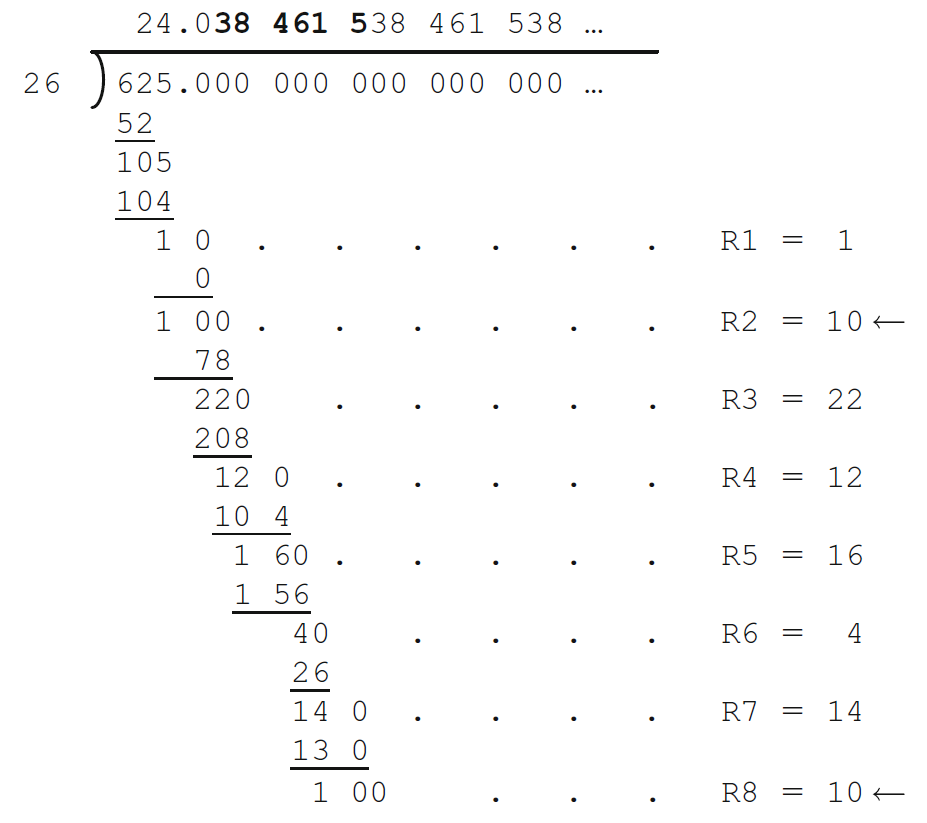
\includegraphics[width=7cm]{img/binary1.PNG}
	\end{center}
	\end{figure}
	
	\pause
	L'algoritmo della divisione e usiamo la notazione $\frac{625}{26} = 24.0\overline{384615}$
\end{frame}

%%%%%%%%%%%%%%%% NEW SLIDE %%%%%%%%%%%%%%%%%%%%
\begin{frame}
   \frametitle{Errori di Approssimazione: Troncamento}
   
	I {\bf numeri razionali} sono i numeri che possono essere rappresentati come rapporti tra numeri interi.
	
	\bigskip
	Ogni numero razionale rappresentato con una notazione posizionale deve avere una forma di ripetizione,
	anche se solitamente non scriviamo la ripetizione di 0 (per esempio, $\frac{1}{625}=0.0016\overline{0}$),
	
	\bigskip
	Nessun oggetto fisico può contenere un numero infinito di elementi. 
	In pratica, per rappresentare un numero razionale quello che viene fatto è di {\it troncare}
	la rappresentazione usando solo le cifre più significative: tutte le cifre meno significative vengono semplicemente ignorate.
	
	\bigskip
	Per esempio, dato $A=\frac{625}{26} = 24.0\overline{384615}$
	\begin{eqnarray*}
	A_1 &=& 24.03  \quad\quad\mbox{troncamento alle 4 cifre più significative} \\
	A_2 &=& 24.0384 \quad \mbox{troncamento a 4 cifre dopo il punto base}
	\end{eqnarray*}
\end{frame}

%%%%%%%%%%%%%%%% NEW SLIDE %%%%%%%%%%%%%%%%%%%%
\begin{frame}
   \frametitle{Errori di Approssimazione: Arrotondamento}

	In alternativa, in modo migliore per rappresentare un numero razionale è di ``arrotondare'' il numero.
	
	\bigskip
	In base 10, la solita regola di arrotondamento è: 
	
	\begin{quote}
	Se la prossima cifra è maggiore o uguale a 5, allora aggiungi 1 alla cifra meno significativa al numero troncato.
	\end{quote}
	
	\bigskip
	Nell'esempio precedente, dato $A=\frac{625}{26} = 24.0\overline{384615}$
	\begin{eqnarray*}
	A_3 &=& 24.04  \quad\quad \mbox{la prima cifra dopo il 3 è 8 ($>5$)} \\
	A_4 &=& 24.0385 \quad  \mbox{la prima cifra dopo il 4 è 6 ($>5$)}
	\end{eqnarray*}
	
	
\end{frame}

%%%%%%%%%%%%%%%% NEW SLIDE %%%%%%%%%%%%%%%%%%%%
\begin{frame}
   \frametitle{Errore di Approssimazione}
   
   Abbiamo due modi di quantificare l'errore tra un numero $A$ e la sua rappresentazione $B$, 
   dove per errore si intende la differenze $e= A - B$:
   
   \begin{enumerate}
   \item Usare l'{\bf errore assoluto in B} che è il modulo dell'errore: 
   $$|A - B|$$
   \pause
   \bigskip
   \item Usare l'{\bf errore relativo in B} che è l'errore assoluto normalizzato: 
   
   $$\frac{|A - B|}{|A|}$$ 
   
   L'errore relativo viene spesso dato in percentuale.
   \end{enumerate}

   
\end{frame}

%%%%%%%%%%%%%%%% NEW SLIDE %%%%%%%%%%%%%%%%%%%%
\begin{frame}
   \frametitle{Esempi}

   	\begin{figure}[h]
	\begin{center}
	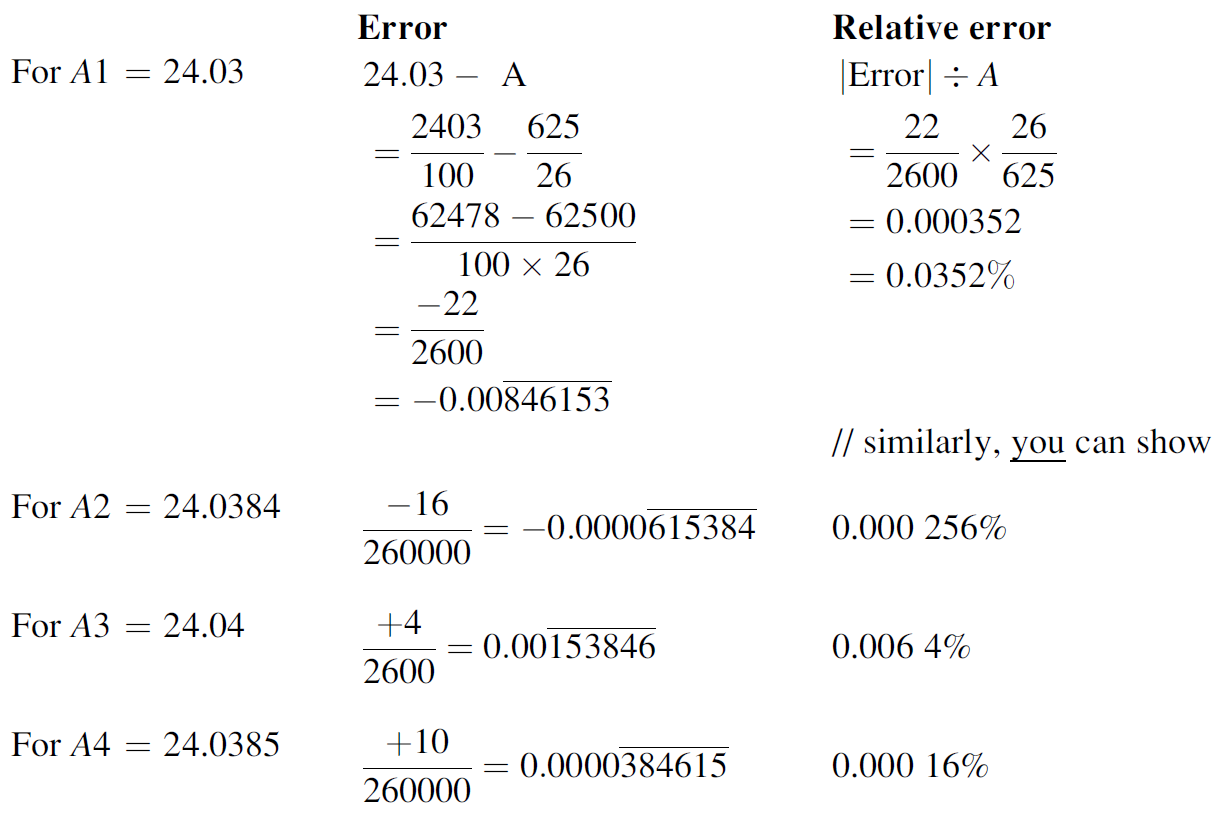
\includegraphics[width=\textwidth]{img/binary2.PNG}
	\end{center}
	\end{figure}
	
\end{frame}

\section {Numerazione Binaria}
\subsection{}
%%%%%%%%%%%%%%%% NEW SLIDE %%%%%%%%%%%%%%%%%%%%
\begin{frame}
   \frametitle{}

    \begin{figure}[h]
	\begin{center}
	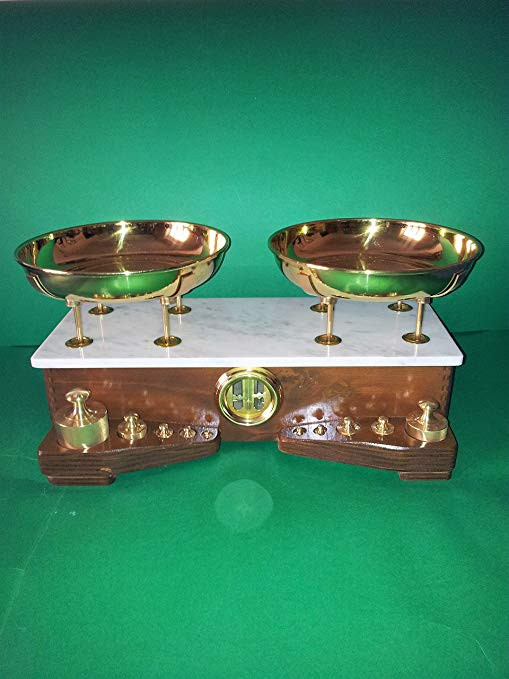
\includegraphics[width=0.5\textwidth]{img/bilancia}
	\end{center}
	\end{figure}
   
\end{frame}

%%%%%%%%%%%%%%%% NEW SLIDE %%%%%%%%%%%%%%%%%%%%
\begin{frame}
   \frametitle{Sistema binario}
   
   I calcolatori sono in grado di gestire due cifre:
   
   $$0, 1$$
   
   Anche con solo due cifre, possiamo usare una notazione posizionale per rappresentare i numeri:
   
   {\small
	\begin{eqnarray*}
	101 111.011 &\mbox{ means } & 1 \times 2^5  + 0\times 2^4 + 1\times 2^3 + 1\times 2^2 + 1\times 2^1 +1 \times 2^0\\
	&&  + 0\times 2^{-1} + 1\times 2^{-2} + 1\times 2^{-3}\\
	&&= 32 + 8 + 4 + 2 + 1 + \frac{1}{4} + \frac{1}{8}\\
	&&= 47 + 0.25 + 0.125 \\
	&& = 47.375
	\end{eqnarray*}}
   
\end{frame}

%%%%%%%%%%%%%%%% NEW SLIDE %%%%%%%%%%%%%%%%%%%%
\begin{frame}
   \frametitle{Somma e prodotto di cifre binarie}

	\begin{center}
	\includegraphics<1->[width=4cm]{img/binary4.PNG}
	\hspace{2cm}
	\includegraphics<2->[width=4cm]{img/binary5.PNG}
	\end{center}

	\uncover<3>{
	Come per la notazione in base 10, anche in base 2 se moltiplichiamo un numero per la base, spostiamo il punto base
    di una posizione verso destra, mentre se dividiamo per la base, 
	spostiamo il punto base di una posizione a sinistra:
	\begin{eqnarray*}
		101111.011 \times 2 &=& 1011110.11\\
		101111.011 \;/\; 2 &=& 10111.1011
	\end{eqnarray*}   
   \bigskip
   Se $k$ è un numero intero positivo, $2^k$ è la cifra 1 seguita da $k$ zeri ($2^4=10000$), e
   $2^{-k}$ è il punto base seguito prima da $(k-1)$ zeri, e poi da uno ($2^{-4}=.0001$). 
}
\end{frame}

%%%%%%%%%%%%%%%% NEW SLIDE %%%%%%%%%%%%%%%%%%%%
\begin{frame}
   \frametitle{}

   \includegraphics<1->[width=\textwidth]{img/binary6.PNG}
\end{frame}

%%%%%%%%%%%%%%%% NEW SLIDE %%%%%%%%%%%%%%%%%%%%
\begin{frame}
   \frametitle{Moltiplicare per due}

   Nell'algoritmo del contadino russo, ad ogni iterazione moltiplichiamo per due il primo numero:

   \bigskip
   \centering   
   \includegraphics<1->[width=\textwidth]{img/binary7.PNG}
\end{frame}


%%%%%%%%%%%%%%%% NEW SLIDE %%%%%%%%%%%%%%%%%%%%
\begin{frame}
   \frametitle{Dividere per due}

   Nell'algoritmo del contadino russo, ad ogni iterazione dividiamo per due il secondo numero e tronchiamo il risultato:
   
   \bigskip
   \centering
   \includegraphics<1->[width=0.8\textwidth]{img/binary8.PNG}
\end{frame}

%%%%%%%%%%%%%%%% NEW SLIDE %%%%%%%%%%%%%%%%%%%%
\begin{frame}
   \frametitle{Moltiplicazione tra numeri binari}

   Se facciamo attenzione, a questo punto dovremmo riconoscere che l'algoritmo del contadino russo non è altro che la solita moltiplicazione svolta in un sistema binario:
   
   \bigskip
   \centering
   \includegraphics<1->[width=\textwidth]{img/binary9.PNG}
\end{frame}

\section {Virgola Mobile}
\subsection{}
%%%%%%%%%%%%%%%% NEW SLIDE %%%%%%%%%%%%%%%%%%%%
\begin{frame}
   \frametitle{Notazione Esponenziale (Normalizzata)}

   La notazione in virgola mobile ({\it floating points}) si basa sulla {\bf Notazione Esponenziale (Normalizzata)} di un numero $x$ in base $\beta$, che è:   
   \begin{eqnarray*}
   x &=& (-1)^s d_0.d_1 d_2 d_3 \dots d_{t-1} \beta^e \\
   &=& (-1)^s (\sum_{i=0,\dots,t-1} d_i \beta^{-i})\,\beta^e\\
   &=& (-1)^s m \beta^e 
   \end{eqnarray*}
   \begin{itemize}
   \item $s$ è il segno di $x$
   \item $\beta$ è un intero $> 1$ e corrisponde alla base
	\item $e$ è l'esponente
	\item $m$ è la mantissa $m = d_0.d_1d_2d_3 \dots d_{t-1}$, in cui $0 \leq d_i \leq \beta-1$
   \end{itemize}

   \bigskip
   {\bf Esempio:} La rappresentazione esponenziale normalizzata in base dieci di $0.00078391$ è $7.8391e^{-4}$
\end{frame}

%%%%%%%%%%%%%%%% NEW SLIDE %%%%%%%%%%%%%%%%%%%%
\begin{frame}
   \frametitle{Insieme dei numeri in virgola mobile}

   Dati due numeri $L$ e $U$ entro cui è compreso l'esponente, possiamo definire il seguente insieme di numeri:
   
   $$
   F(\beta, t, L, U) := \{0\} \cup \{x \mid (-1)^s (\sum_{i=0,\dots,t-1} d_i \beta^{-i})\,\beta^e, L \leq e \leq U\}
   $$
   
   Si osservi che:
   \begin{itemize}
   \item Si ha che $x \in F$ se e solo se $-x \in F$
   \item Per ogni $x \in F, x \neq 0$, si ha che:
   
   $$x_{min} = \beta^{L} \leq |x| \leq \beta^{U} (2 - \beta^{-t+1}) = x_{max}$$
   \end{itemize}
\end{frame}

%%%%%%%%%%%%%%%% NEW SLIDE %%%%%%%%%%%%%%%%%%%%
\begin{frame}
   \frametitle{Esempio: $F(\beta=2,t=3,L=-1,L=2)$}

   Rappresentazione grafica dei numeri 16 (più lo 0) normalizzati (ovvero con $d_0>0$) contenuti nell'insieme:

   $$F(\beta=2,t=3,L=-1,L=2)$$

	\vspace{1cm}
   \bigskip
   \centering
   \includegraphics<1->[width=\textwidth]{img/binary10.PNG}
   
\end{frame}

%% TODO: Aggiungi numeri normalizzati solo per e=L

%%%%%%%%%%%%%%%% NEW SLIDE %%%%%%%%%%%%%%%%%%%%
\begin{frame}
   \frametitle{Standard IEEE 754}

   Sui calcolatori esistono due notazioni standard per i numeri in virgola mobile:
   
   \begin{enumerate}
   \item Singola precisione, usa $t=32$ bits: 1 bit di segno, 8 bits per l’esponente, e 23 per la mantissa
   
   \bigskip
   \begin{center}
   \includegraphics<1->[width=0.5\textwidth]{img/binary11.PNG}
   \end{center}
   
   \bigskip
   \item Doppia precisione, usa $t=64$ bits: 1 bit di segno, 11 bits per l’esponente, e 52 per la mantissa
   \end{enumerate}
   
\end{frame}

%%%%%%%%%%%%%%%% NEW SLIDE %%%%%%%%%%%%%%%%%%%%
\begin{frame}
   \frametitle{Standard IEEE 754: Esempio}

   \begin{center}
   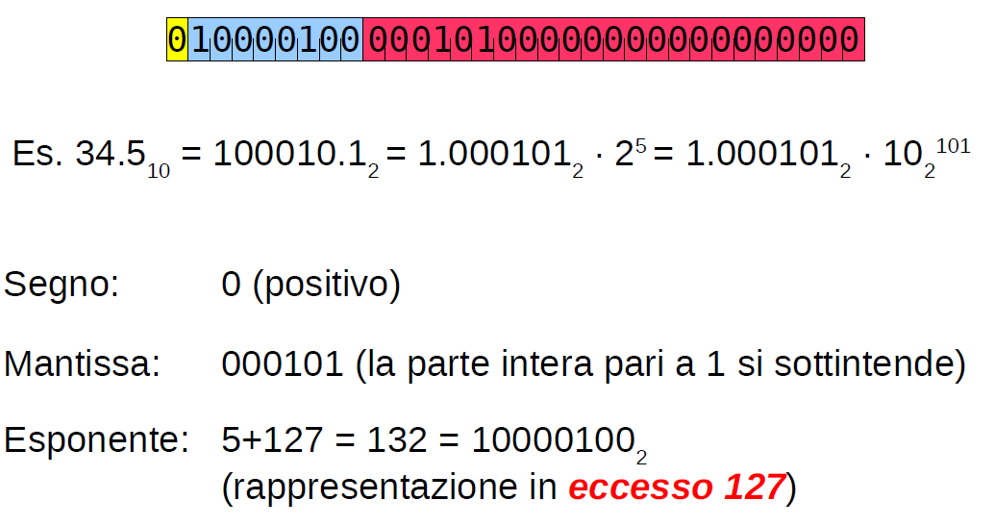
\includegraphics[width=\textwidth]{img/binary12.PNG}
   \end{center}
\end{frame}


%%%%%%%%%%%%%%%% NEW SLIDE %%%%%%%%%%%%%%%%%%%%
\begin{frame}
   \frametitle{Riferimenti}

   \begin{itemize}
   \item Tom Jenkyns, Ben Stephenson. Fundamentals of Discrete Math for Computer Science: A Problem-Solving Primer (Capitolo 1). Springer, 2012.
   
   \bigskip
   \item David Goldberg. {\it What every computer scientist should know about floating-point arithmetic}. 
   ACM Computing Surveys (CSUR). Vol 23(1), pp. 5-48.
   \end{itemize}
\end{frame}
\end{document}
